\documentclass{article}
\usepackage[style=apa]{biblatex}


\bibliography{article}

\addbibresource{\jobname.bib}
%\AtEveryBibitem{\printfield{note}\clearfield{note}\item}


\usepackage{subcaption}
\usepackage[margin=1in]{geometry}
\usepackage{amsmath}
\usepackage{tikz}
\usetikzlibrary{angles}
\usetikzlibrary{arrows.meta}
\usetikzlibrary{automata}
\usetikzlibrary{calc}
\usetikzlibrary{chains}
\usetikzlibrary{decorations.pathreplacing}
\usetikzlibrary{positioning}
\usetikzlibrary{quotes}
\usepackage{graphicx} % Required for inserting images
\usepackage[T1]{fontenc}
\usepackage{beramono}
\usepackage{courier}
\usepackage{listings}
\usepackage{xpatch}
\usepackage{realboxes}
\usepackage{titlesec}
\usepackage{xcolor}
\usepackage{minted}

\definecolor{LightGray}{gray}{0.97}


\setcounter{secnumdepth}{4}


\titleformat{\paragraph}
{\normalfont\normalsize\bfseries}{\theparagraph}{1em}{}
\titlespacing*{\paragraph}
{0pt}{3.25ex plus 1ex minus .2ex}{1.5ex plus .2ex}


\lstdefinelanguage{none}{
  identifierstyle=
}

\definecolor{mygreen}{rgb}{0,0.8,0}
\definecolor{mygray}{rgb}{0.5,0.5,0.5}
\definecolor{mymauve}{rgb}{0.58,0,0.82}
\definecolor{mygray}{rgb}{0.94,0.94,0.94}



%%% Wrap colorbox around lstinline %%%
\makeatletter
\xpretocmd\lstinline{\Colorbox{mygray}\bgroup\appto\lst@DeInit{\egroup}}{}{}
\makeatother
%%%%%%%%%%%%%%%%%%%%%%%%%%%%%%%%%%%%%%

\lstset{ 
  backgroundcolor=\color{mygray},   % choose the background color; you must add \usepackage{color} or \usepackage{xcolor}; should come as last argument
  breakatwhitespace=false,         % sets if automatic breaks should only happen at whitespace
  basicstyle=\ttfamily,
  breaklines=true,                 % sets automatic line breaking
  captionpos=b,                    % sets the caption-position to bottom
  commentstyle=\color{mygreen},    % comment style
  deletekeywords={...},            % if you want to delete keywords from the given language
  escapeinside={\%*}{*)},          % if you want to add LaTeX within your code
  extendedchars=true,              % lets you use non-ASCII characters; for 8-bits encodings only, does not work with UTF-8
  firstnumber=1000,                % start line enumeration with line 1000
  frame=none,	                   % adds a frame around the code
  keepspaces=true,                 % keeps spaces in text, useful for keeping indentation of code (possibly needs columns=flexible)
  keywordstyle=\color{blue},       % keyword style
  language=Octave,                 % the language of the code
  morekeywords={*,...},            % if you want to add more keywords to the set
  numbers=none,                    % where to put the line-numbers; possible values are (none, left, right)
  numbersep=5pt,                   % how far the line-numbers are from the code
  numberstyle=\tiny\color{red}, % the style that is used for the line-numbers
  rulecolor=\color{black},         % if not set, the frame-color may be changed on line-breaks within not-black text (e.g. comments (green here))
  showspaces=false,                % show spaces everywhere adding particular underscores; it overrides 'showstringspaces'
  showstringspaces=false,          % underline spaces within strings only
  showtabs=false,                  % show tabs within strings adding particular underscores
  %stepnumber=2,                    % the step between two line-numbers. If it's 1, each line will be numbered
  stringstyle=\color{mymauve},     % string literal style
  tabsize=2,	                   % sets default tabsize to 2 spaces
  title=\lstname                   % show the filename of files included with \lstinputlisting; also try caption instead of title
}

\definecolor{codegreen}{rgb}{0,0.6,0}
\definecolor{codegray}{rgb}{0.5,0.5,0.5}
\definecolor{codepurple}{rgb}{0.58,0,0.82}
\definecolor{backcolour}{rgb}{0.95,0.95,0.92}

\lstdefinestyle{mystyle}{
    backgroundcolor=\color{backcolour},   
    commentstyle=\color{codegreen},
    keywordstyle=\color{magenta},
    numberstyle=\tiny\color{codegray},
    stringstyle=\color{codepurple},
    basicstyle=\ttfamily\footnotesize,
    breakatwhitespace=false,         
    %breaklines=true,                 
    %captionpos=b,                    
    keepspaces=true,                 
    numbers=left,                    
    numbersep=5pt,                  
    showspaces=false,                
    showstringspaces=false,
    showtabs=false,                  
    tabsize=2
}

\lstset{style=mystyle}

\tikzset{
box/.style={draw,
  inner sep=0.3cm,
    minimum height=1.75cm,
    align=center},
cbox/.style={draw,
  font=\ttfamily,},
}
\tikzset{invisible/.style={minimum width=0mm,inner sep=0mm,outer sep=0mm}}

\title{Implementation and comparison of register allocation to translate \lstinline!LLVM--! to x86}
\author{William Welle Tange}
\date{2023}


\begin{document}

\maketitle

\tableofcontents
\newpage

%% TODO: tjek hvad LLVM gør %%


%\texttt{LLVM-{}-2}
%* skab så mange underpunkter som muligt
    %* jo mindre man skal overskue af gangen jo lettere er det at komme i gang med at skrive
    

\section{Introduction}

Compilation refers to the process of translating from one language to another, most often from a high-level programming language intended for humans to work with, to machine- or bytecode intended to be executed on a target architecture. This process can be divided into several distinct phases, which are grouped into one of two stages colloquially referred to as the \textit{frontend} and \textit{backend}, the former translating a high-level programming language to an \textit{intermediate representation} (IR) and the latter translating IR to executable machine code of a target architecture or bytecode of a target \textit{virtual machine} (VM).



\begin{figure}[h]
  \centering
  \resizebox{0.8\textwidth}{!}{
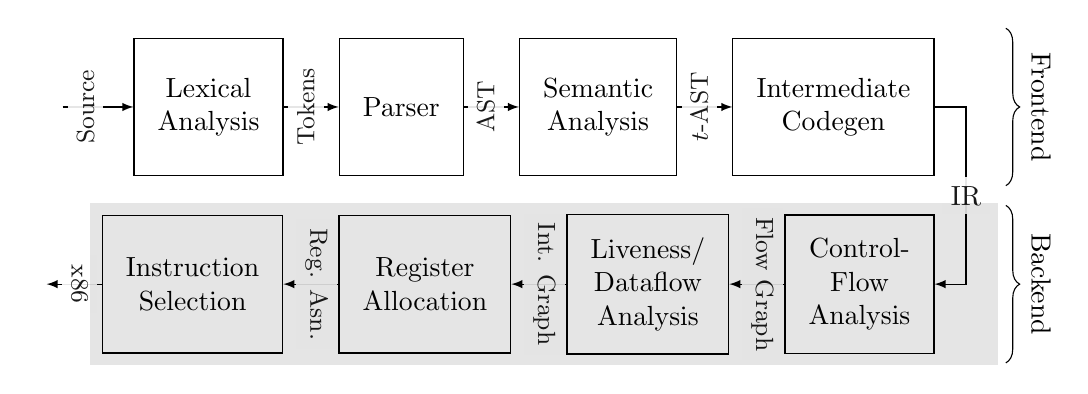
\begin{tikzpicture}


  % Nodes
  \node [box, left, align=center] (incg) at (0,2.25) {Intermediate\\Codegen};
  \node [box, left=0.7 of incg, align=center] (semant) {Semantic\\Analysis};
  \node [box, left=0.7 of semant, align=center] (parse) {Parser};
  \node [box, left=0.7 of parse, align=center] (lex) {Lexical\\Analysis};
  \node [ left=0.9 of lex, align=center] (entry) {};
  \node [box, left, align=center] (cfa) at (0,0) {Control-\\Flow\\Analysis};
  \node [box, left=0.7 of cfa, align=center] (lva)  {Liveness/\\Dataflow\\Analysis};
  \node [box, left=0.7 of lva, align=center] (alloc)  {Register\\Allocation};
  \node [box, left=0.7 of alloc, align=center] (x86)  {Instruction\\Selection};
  \node [ left=0.70 of x86, align=center] (exit) {};

  % Edge with right-angle corners
  \draw [-latex] (entry.east) -- (lex.west)  node [near start,pos=0.325,rotate=90,fill=white,opacity=0.9] {\small Source};
  \draw [-latex] (lex.east) -- (parse.west)  node [midway,pos=0.4,rotate=90,fill=white,opacity=0.9] {\small Tokens};
  \draw [-latex] (parse.east) -- (semant.west)  node [midway,pos=0.4,rotate=90,fill=white,opacity=0.9] {\small AST};
  \draw [-latex] (semant.east) -- (incg.west)  node [midway,pos=0.4,rotate=90,fill=white,opacity=0.9] {\small \(t\)-AST};
  \draw [-latex] (incg.east) -- +(0.4,0) |- node[pos=0.25,fill=white,opacity=0.9] {IR} (cfa.east);
  \draw [-latex] (cfa.west) -- (lva.east)  node [midway,pos=0.4,rotate=-90,fill=white,opacity=0.9] {\small Flow Graph};
  \draw [-latex] (lva.west) -- (alloc.east)  node [midway,pos=0.4,rotate=-90,fill=white,opacity=0.9] {\small Int. Graph};
  \draw [-latex] (alloc.west) -- (x86.east)  node [midway,pos=0.4,rotate=-90,fill=white,opacity=0.9] {\small Reg. Asn.};
  \draw [-latex] (x86.west) -- (exit.east)  node [midway,pos=0.4,rotate=-90,fill=white,opacity=0.9] {\small x86};

  % backend outline
  \fill [opacity=0.1] ([shift={(-0.15,-0.15)}]x86.south west) rectangle ([shift={(0.8,0.15)}]cfa.north east);

  \draw [decorate,decoration={brace,amplitude=5pt,mirror,raise=4ex}]
    (0.3,-1) -- (0.3,1) node[midway,xshift=3em,rotate=-90]{Backend};
  \draw [decorate,decoration={brace,amplitude=5pt,mirror,raise=4ex}]
    (0.3,1.25) -- (0.3,3.25) node[midway,xshift=3em,rotate=-90]{Frontend};
\end{tikzpicture}}
\caption{Compiler phases, backend highlighted}
\end{figure}
Most operations of a general-purpose programming language are translated to a set of control, logic, and arithmetic instructions to be executed sequentially on a computer processor: a single circuit/chip, referred to as the \textit{central processing unit} (CPU), the design of which has varied and evolved over time.

Most CPUs are \textit{register machines}, in that they use a limited set of \textit{general-purpose registers} (GPRs) to store working values in combination with \textit{random access memory} (RAM) for mid-term, and other I/O peripherals for long-term storage. This can largely be attributed to performance, as register machines routinely outperform \textit{stack machines} \parencite{ShiYunhe2008VmsS} that are often used in VMs.
Because of the limited amount of GPRs available simultaneously, a crucial part of the backend stage for an optimizing compiler is assigning each variable  of the source program to a GPR in such a way that maximizes performance without sacrificing correctness.

The process of assigning each variable to a GPR is referred to as \textit{register allocation}, and can be approached in several different ways. This paper will seek to implement graph coloring and linear scan and evaluate them in terms of runtime performance after compilation. %% TODO: compare with time-complexity/compile-time duration?
The primary sources will be \textit{Modern Compiler Implementation in ML} \parencite{tiger} and \textit{Compilers: Principles, techniques, and tools} \parencite{dragon}, in addition to publications concerning the linear scan approach.


%* overfladisk intro til hvad helvede register allokering er og hvorfor
    %* hovedtræk
%* rudimentær del af compilation/oversættelse fra high-level sprog til x86 er register allokering
    %* projektet er skridtet videre fra compilers kurset
    %* siger hvad jeg står ovenpå/bygger på
%snak om hvorfor jeg valgte llvm/ssa frem for x86 til global register llocation


%\section{Review of Literature}

%The two primary sources are the \textit{Modern Compiler Implementation in ML} \cite{tiger} and Dragonbook \cite{dragon}, in addition to scientific publications concerning the linear scan approach.



\section{Control Flow Analysis}

% TODO: figure out what traces are
% TODO: mention dominators etc.


The backend of a compiler takes some form of IR as input, usually a linear sequence of instructions for each separate function. This representation is close to the level of an actual processor by design, but it isn't immediately useful for the further analysis steps needed to generate optimized code for the target architecture. %%(FIXME: why not?)
The control flow of a given program refers to the order in which instructions are executed. While the flow of most instructions is linear, in the sense that the next instruction executed is located immediately after, some transfer the flow of execution elsewhere or even terminate it. %% FIXME: why is this important?

% mention basic block early on, they're a contiguous sequence of instructions that do not transfer control flow

A continuous flow of instructions is referred to as a \textit{basic block}, defined as a sequence of instructions with no branches in or out except for the first instruction (referred to as a \textit{leader}, immediately following either the function entry or label) and the last (referred to as a \textit{terminator}, as it either terminates or transfers the flow of execution). %These are often referred to as terminators and can be thought of as an entirely different categoriy of instructions. % TODO: måske drop 'can be thought of'

Basic blocks represent a single node in a \textit{control flow graph} (CFG), which is a directed graph whose edges denote transfer of  control flow. The unconditional branch terminator always transfers control flow to the block labelled, meaning only one successor will follow, whereas conditional branching could transfer to either of the two, but because control flow analysis is not concerned with data, it simply adds both as successors. % TODO: rets 
While each block has 0-2 immediate successors, the amount of predecessors is unbounded as the amount of branches targeting a specific leader is unlimited.

\begin{figure}[h]
  \centering
  \begin{subfigure}{0.48\textwidth}
  \centering
  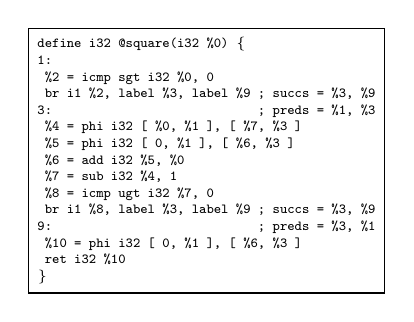
\begin{tikzpicture}
    \node [cbox, font=\ttfamily\tiny, align=left] (cfa) at (0,0) {define i32 @square(i32 \%0) \{\\1:\\\ \%2 = icmp sgt i32 \%0, 0\\\ br i1 \%2, label \%3, label \%9\ ; succs = \%3, \%9\\3:\ \ \ \ \ \ \ \ \ \ \ \ \ \ \ \ \ \ \ \ \ \ \ \ \ \ \ \ ; preds = \%1, \%3\\\ \%4 = phi i32 [ \%0, \%1 ], [ \%7, \%3 ]\\\ \%5 = phi i32 [ 0, \%1 ], [ \%6, \%3 ]\\\ \%6 = add i32 \%5, \%0\\\ \%7 = sub i32 \%4, 1\\\ \%8 = icmp ugt i32 \%7, 0\\\ br i1 \%8, label \%3, label \%9\ ; succs = \%3, \%9\\9:\ \ \ \ \ \ \ \ \ \ \ \ \ \ \ \ \ \ \ \ \ \ \ \ \ \ \ \ ; preds = \%3, \%1\\\ \%10 = phi i32 [ 0, \%1 ], [ \%6, \%3 ]\\\ ret i32 \%10\\\}};
  \end{tikzpicture}
  \end{subfigure}
  \begin{subfigure}{0.48\textwidth}
  \centering
  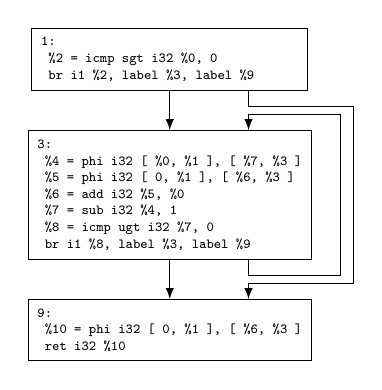
\begin{tikzpicture}
    \node [cbox, font=\ttfamily\tiny, align=left] (a) at (0,0) {1:\\\ \%2 = icmp sgt i32 \%0, 0\\\ br i1 \%2, label \%3, label \%9\ \ \ \ \ \ \ };
    \node [cbox, font=\ttfamily\tiny, align=left, below=0.5cm of a] (b) {3:\\\ \%4 = phi i32 [ \%0, \%1 ], [ \%7, \%3 ]\\\ \%5 = phi i32 [ 0, \%1 ], [ \%6, \%3 ]\\\ \%6 = add i32 \%5, \%0\\\ \%7 = sub i32 \%4, 1\\\ \%8 = icmp ugt i32 \%7, 0\\\ br i1 \%8, label \%3, label \%9};
    \node [cbox, font=\ttfamily\tiny, align=left, below=0.5cm of b] (c) {9:\\\ \%10 = phi i32 [ 0, \%1 ], [ \%6, \%3 ]\\\ ret i32 \%10};

    \node[right= 1cm of a.south, invisible] (ac1)  {};
    \node[below= 0.166667cm of ac1, invisible] (ac2)  {};
    \node[right= 1.333333cm of ac2, invisible] (ac3)  {};
    \node[right= 1cm of c.north, invisible] (ac6)  {};
    \node[above= 0.166667cm of ac6, invisible] (ac5)  {};
    \node[right= 1.333333cm of ac5, invisible] (ac4)  {};

    \node[right= 1cm of b.north, invisible] (bb1)  {};
    \node[above= 0.166667cm of bb1, invisible] (bb2)  {};
    \node[right= 1.166667cm of bb2, invisible] (bb3)  {};
    \node[right= 1cm of b.south, invisible] (bb6)  {};
    \node[below= 0.166667cm of bb6, invisible] (bb5)  {};
    \node[right= 1.166667cm of bb5, invisible] (bb4)  {};

    %\node[right=2.5cm of ab, invisible] (abr)  {};
    %\node[right=2.5cm of bc, invisible] (bcr)  {};
  \draw [-latex] (a) -- (b);
  %\draw [-latex] (a) to[out=-15,in=15] (c);
  \draw [-latex] (b) -- (c);


  \draw          (ac1.center) -- (ac2.center) -- (ac3.center) -- (ac4.center) -- (ac5.center);
  \draw [-latex] (ac5.center) -- (ac6.center);

  \draw          (bb2.center) -- (bb3.center) -- (bb4.center) -- (bb5.center) -- (bb6.center);
  \draw [-latex] (bb2.center) -- (bb1.center);
  %\draw [-latex] (c.north) to[bend right=1000] (b.north);
  %\draw  (a.south) to  (ab);
  %\draw  (ab) to  (abr);
  %\draw  (abr) to  (bcr);
  %\draw  (bcr) to  (bc);
  %\draw  (ab) to  (bc);
  %\draw [-latex]  (bc) to [out=180,in=70] (c.north);
  \end{tikzpicture}
  \end{subfigure}
  \hfill
  \caption{CFG of \lstinline!@square! of \lstinline!square.ll!} % FIXME: not entirely correct (square.ll is @main)
\end{figure}

%These instructions are referred to as \textit{terminators}, as they potentially terminate a contiguous flow of execution. This subset of instructions can be further divided into \textit{branch instructions} and those concerned with handling the callstack in function/subroutine management.

%These so-called \textit{branch instructions} that alter the flow of execution are further c



% FIXME: introducer phi nodes og nævn dominators i CFA afsnittet





%hence a \textit{control flow graph} is derived from these. A terminator will branch elsewhere to continue execution. The destination of this has to be an annotated by a label, hence labels \textit{initiate} blocks.

\subsection{Building a graph}

\subsection{Parameterized over individual instructions}

\subsection{Parameterized over basic blocks}


With an input stream of instructions 

%* description of blocks, how they connect etc.

Each function defined in an LLVM program is constructed with the help of

\section{Liveness Analysis}

% * Different approaches:
%   * Naive/greedy 
%   * Dataflow analysis 
%     * forward must
%     * backwards may
%   * linear scan
%
%  TODO: comment on interrupts

Translating IR with an unbounded number of variables to a CPU with a bounded number of registers involves the process of assigning each variable a register such that no value that can be used in the future is overwritten. %Therefore, any variable that may be used in the future is considered \textit{live}, and said to be in interference with any other variable live at any intersecting point.
Variables that are in use at a given program point are considered \textit{'live'}, and although variables can be assigned the same register, %if they are not in interference
variables that are live at the same time (i.e. at intersecting program points) cannot, in which case they are also said to be in interference with one another.
 Variables that are not in interference can be assigned the same register, and finding the precise points at which any variable is live is trivial for linear sequences of instructions. However, when conditional branching is introduced, deriving the path of execution becomes undecidable because of the halting problem. % TODO: finish this sentence

Suppose a function that calls another:

\begin{lstlisting}[language=LLVM,firstnumber=1]
define i32 @countcall(i32 %x0) {
  %x1 = add i32 %x0, 1
  call ptr @subproc()
  ret i32 %x1
}
\end{lstlisting}
Because of the halting problem, static analysis cannot determine if the call to \lstinline!@subproc! will return for every possible implementation.  %which may or may not return control to the calling function:
 So when assigning \lstinline!%x1! a register it is undecidable whether the variable must be live in the last return instruction, i.e. needs to live across the call to another function which can overwrite several registers depending on calling conventions. Because of this, any sound approach to liveness analysis will be an approximation.

 % TODO: maybe find a better exampple with a better assignment that computer can't find?
 % TODO: maybe mention exponential brute force algorithms?

A sound albeit very naive approach is to consider every variable live at every program point, such that every variable is in interference with one another, producing a fully connected interference graph. % FIXME: find a place for: This generally isn't a very performant approach in terms of execution 
Such a heuristic is greedy in the sense that it picks an assignment known to be safe for the least amount of preprocessing work possible. However, this can be a very inefficient assignment at runtime: a number of \(n\)  variables greater than \(k\) working registers causes \(n-k\) variables to be spilled to memory, % TODO: skal der stå stack?
which can greatly reduce performance, but  allows for translation in constant time. %FIXME: is this even true?

\newpage
\subsection{Dataflow Analysis}

% FIXME: beskriv use, def osv. sets tidligere!

Another approach, which is a much more precise approximation, is a specific variant of the dataflow analysis as described in \textit{Modern Compiler Implementation in ML} (\cite{tiger}) and \textit{Compilers: Principles, Techniques, and Tools} (\cite{dragon}). In general, dataflow analysis is the process of finding the possible paths in which data may propagate through different branches of execution.  While several applications of this exist (like constant propagation, reaching defnitions, available expressions etc.), one that is immediately beneficial in the case of liveness analysis is one that traverses a CFG in the reverse order of execution (i.e.  \textit{backwards} flow), and extracts any variable that \textit{may} be used in execution (also referred to as \textit{backwards may} analysis). % FIXME: forklar hvorfor List.rev ikke udgør backwards flow

This algorithm calculates which program points each variable may be accessed from with some conservative constraints known to maintain correctness. Specifically, these are the transfer and control-flow constraints. %, the former of which must satisfy a transfer function a

The transfer constraint is based on a \textit{transfer function} that describes how liveness is affected across instructions. For each instruction, there is a transfer function that describes how liveness changes from one point to the one immediately after. For example, as an arithmetic operation needs to be assigned a new temporary variable, the liveness of a new variable is propagated to all  instructions  executed subsequently. This is done by applying the transfer function to the current \textit{live-out} set to stop further propagation of variables defined by the currently visited instruction. % TODO: In fact, because the IR is in SSA form, the only time 
\begin{align}\label{flowin}
  \mathit{in}\left[n\right] &= \mathit{use}\left[n\right] \cup (\mathit{out}\left[n\right] - \mathit{def}\left[n\right])
\end{align}
Control-flow constraints on the other hand propagate the use of variables to previously executed instructions, expecting these to be defined somewhere further up the CFG. This is done by propagating the union of the \textit{live-in} set associated with all immediate successor nodes. This is also referred to as the \textit{meet operator}, whose operator depends on the type of dataflow alanysis as well, but for liveness analysis a union is performed on the previos \textit{live-in} variables.
\begin{align}\label{flowout}
  \mathit{out}\left[n\right] &= \bigcup_{s\in \mathit{succ}\left[n\right]} \mathit{in}\left[s\right]
\end{align}
%in order to maintain correctness by iteratively applying a set of constraints until a fixed point is reached.
%These constraints are applied to the \(\textit{live-in}\left[i\right]\) and  \(\textit{live-out}\left[i\right]\) sets for every instruction \(i\). Both are initialized to the empty set \(\emptyset\).
%The dataflow analysis approach builds the set of variables that 
%Each type of instruction has some semantic attributes that are applied to the system state upon execution. This change is also referres to as a \textit{transfer function} as it transitions from one state to another.
%can be thought of as a \textit{transfer function} in terms of liveness, denoting which variables may be live before and after execution.
Initially, two sets are associated with each instruction: the \textit{live-in} and \textit{live-out} sets, which are the sets of variables that are live respectively before and after execution. Then the following two equations are applied iteratively until a fixed point is reached, i.e. a point in which neither \(\mathit{in}[n]\) or \(\mathit{out}[n]\) is changed for all \(n\) instructions.

% TODO: onwards!


%builds sets of \textit{live-in} and  \textit{live-out} variable for each instruction.

% must be assigned in such a way that ensures its availability at every subsequent use throughout execution.

%Variables can be assigned the same register if they are not in use at the same time, so variables that are in use at the same time are said to be in interference with one another.

%Liveness analysis is the process of finding the program points at which a variable is live. This serves the function of determining which variables are live simultaneously, i.e. in conflict/interference with one another, so cannot be assigned the same physical register without overwriting the value of one another.



%Another approach that takes CFG into consideration is that of 


%These can be derived recursively by iteratively applying so-called \textit{dataflow equations} to each node in a \textit{control-flow graph} (CFG) until a stable state/fixed point is reached.

%The algorithm described in \textit{Modern Compiler Implementation in ML} \cite{tiger} and \cite{dragon} is based on the following equations for the live-in and live-out variables respectively:
%where \(use\left[n\right]\) is the set of all dependent variables, \(def\left[n\right]\) is the set of all variables defines and \(succ\left[n\right]\) is the set of all immediate successor nodes of \(n\).

%The structure of the CFG is inherently vague as both   \cite{tiger} and \textit{Compilers : Principles, Techniques, and Tools} \cite{dragon}, while based on the same underlying % TODO: fix references
%conceptions of dataflow, have different approaches to nodes of a CFG, with the former taking each individual instruction into consideration and the latter each basic block. Either of these approaches are sound 


% TODO: try int set instead of symbols

%The purpose of liveness analysis is to determine which variables are live at which program point, which in turn is used to 

%\subsubsection{Implementation}

The simplest ones to implement are the \lstinline!def! and \lstinline!use! functions, as all of the values of interest are located immediately within the instruction itself and not hidden behind some layer of indirection:
\begin{minted}[linenos,bgcolor=LightGray]{ocaml}
let def (s : S.SS.t) (insn : Cfg.insn) =
  match insn with Insn (Some dop, _) -> S.SS.add dop s | _ -> s

let use (s : S.SS.t) (insn : Cfg.insn) =
  let op o s = match o with Ll.Id i -> S.SS.add i s | _ -> s in
  let po s o = op o s in
  match insn with
  | Insn (_, AllocaN (_, (_, o)))
  | Insn (_, Bitcast (_, o, _))
  | Insn (_, Load (_, o))
  | Insn (_, Ptrtoint (_, o, _))
  | Insn (_, Sext (_, o, _))
  | Insn (_, Trunc (_, o, _))
  | Insn (_, Zext (_, o, _)) ->
      op o s
  | Insn (_, Binop (_, _, l, r))
  | Insn (_, Icmp (_, _, l, r))
  | Insn (_, Store (_, l, r)) ->
      op l s |> op r
  | Insn (_, Call (_, _, args)) -> List.map snd args |> List.fold_left po s
  | Insn (_, Gep (_, bop, ops)) -> List.fold_left po (op bop s) ops
  | Insn (_, Select (c, (_, l), (_, r))) -> op c s |> op l |> op r
  | Insn (_, PhiNode (_, ops)) -> List.map fst ops |> List.fold_left po s
  | Term (Ret (_, Some o) | Cbr (o, _, _)) -> op o s
  | _ -> s
\end{minted}
Where \lstinline!S.SS! is a \lstinline!Set.S! module built over the \lstinline!symbol! type found in \lstinline!lib/symbol.ml!:
\begin{minted}[linenos,bgcolor=LightGray]{ocaml}
type symbol = string * int
(* ... *)
module SS = Set.Make (struct
  type t = symbol
  let compare (_, n1) (_, n2) = compare n1 n2
end)
type set = SS.t
\end{minted}
With the actual fixed-point iteration performed as follows:
\begin{minted}[linenos,bgcolor=LightGray]{ocaml}
let dataflow (insns : Cfg.insn list) (ids : Cfg.G.V.t array) (g : Cfg.G.t) =
  let insns = List.mapi (fun i v -> (i, v)) insns |> List.rev in
  let in_ = Array.init (List.length insns) (fun _ -> S.SS.empty) in
  let out = Array.init (List.length insns) (fun _ -> S.SS.empty) in
  let rec dataflow () =
    let flowout = (* ... *)
    let flowin = (* ... *)
    let flow changed insn = changed || flowout insn || flowin insn in
    if List.fold_left flow false insns then dataflow () else (in_, out)
  in
  dataflow ()
\end{minted}
The \texttt{flowin} function correponds to the \textit{live-in} equation \eqref{flowin} and is implemented as follows:
\begin{minted}[linenos,bgcolor=LightGray]{ocaml}
let flowin (i, insn) =
  let newin = S.SS.union (use insn) (S.SS.diff out.(i) (def insn)) in
  let changed = not (S.SS.equal newin in_.(i)) in
  if changed then in_.(i) <- newin;
  changed
\end{minted}
And the \texttt{flowout} function which correponds to the \textit{live-out} equation \eqref{flowout} implemented as follows:
\begin{minted}[linenos,bgcolor=LightGray]{ocaml}
let flowout (i, _) =
  let newout =
    let succ = Cfg.G.succ g ids.(i) in
    List.fold_left
      (fun s v -> S.SS.union s in_.(Cfg.G.V.label v))
      S.SS.empty succ
  in
  let changed = not (S.SS.equal newout out.(i)) in
  if changed then out.(i) <- newout;
  changed
\end{minted}


\subsection{Interference Graph}

The purpose for conducting dataflow analysis as above is finding variables that may be assigned the same register. This is done by building an interference graph, which is an undirected graph, whose nodes represent variables and edges signify interference between them, i.e. variables \(a\) and \(b\) live at overlapping program points is represented with an edge \((a,b)\).


Constructing an interference graph only depends on the \textit{live-out} set and type of instruction. If the instruction defines a variable, said variable is in interference with all variables in the \textit{live-out} set. There is one exception however: according to the Appel text, move instructions (i.e. phi nodes in the case of SSA form) are given special consideration. The purpose of phi nodes is to copy/move a certain value from a certain predecessor, so they are not necessarily in conflict for being live at the same time. Rather it would often benefit if they were assigned the same register to spare unnecessary moves. % TODO: uddyb hvorfor de ikke er i interference?


Because of this, for any phi node of the form 
\[
  a = \Phi (b_1, ..., b_n)
\]
add edges to all \textit{live-out} variables not in \(B\)
\[
  \forall b_j \in (\mathit{out}[i] \setminus B), \mathit{add\_edge}(a, b_j) \text{ where } B = \{b_1, ..., b_n\}
\]
For any other instruction the defines a variable \(a\)
\[
  \forall b_j \in B, \mathit{add\_edge}(a, b_j)
\]
Although the Appel text notes interference with concrete registers as well as overlapping variables, this isn't considered in this implementation.



%\section{CFG -> INTERF}

%* describe the dataflow algorithm from the book
%* describe the interference criteria from the book

%\section{INTERF -> DOT}

%* ez ???

%\section{INTERF -> DOT/Assignment}

%* list of methods for coalescing/allocating:
%   * ocamlgraph builtin
%   * greedy 
%   * briggs
%   * george
%   * welsh-powell?
\section{Graph Coloring}
Once an interference graph is constructed, the actual assignments can be found using graph coloring. Although this has long been known to be NP-complete, the heuristic as introduced in both the Appel and Aho et al. texts is a linear time approximation to this problem. It is based on an iterative approach wherein nodes known to be colorable are removed until either an empty graph remains in which case the original graph \(G\) is \(k\)-colorable  or nodes with more than \(k\) neighbours remain, in which case a node is chosen to be spilled to the stack and removed. This is then repeated.

Let \(k\) be the number of working registers available on the target architecture. After building the interference graph \(G\), a node \(n\) with fewer than \(k\) neighbors is chosen. As \(n\) has at most \(k-1\) neighbors, it can be removed safely, effectively simplifying \(G\). It is pushed to a stack in order to preserve the order in which they are removed so that \(G\) can be rebuilt and the corresponding registers can be assigned correctly once a \(k\)-colorable assignment is found.
%  (i.e. \(\mathit{deg}(n) < k\))

%It must hold that \(G-\{n\}\) is \(k\)-colorable if \(G\) is \(k\)-colorable 

\subsection{Coloring by simplification}

%% TODO
%* optimistic coloring
\subsection{Coalescing}

Coalescing is the process of eliminating moves/copies of data from one GPR to another by combining their interference graph nodes. This is similar to but  not the same as  the lack of interference edges between variables subject to move operations. This is because variables \(a\) and \(b\) may still be assigned different registers or even spilled if,  for instance, either of them are of significant degree. Coalescing joins nodes \(a\) and \(b\) to node \(ab\) preserving the edges of both to maintain soundness.

Since all edges are preserved, the resulting node \(an\) may be of a much higher degree. Because to this, only strategies that produce a \(k\)-colorable graph are worth considering as worth considering as additional spills negate the purpose entirely.

\section{Linear Scan}

%Write about Appel book.

%Write about SSA form liveness analysis. 

%Keywords: program points, dataflow equations, fixed point




%* todo: ssa/llvm vs appel analysis
%* henvis til blog posts som archive
%    * så tæller det som litteratur
%* tag essensen ud af hvad der bliver sagt i teksten
    %* som er relevant for mit arbejde
%
%* HENVIS TIL KAPITEL 19 OM SSA FORM
%
%* linear scan approach
%
%* snak om hvilke dele af bogen i hvilken rækkefølge
%
%Appel (208p):
%*   Translation To Intermediate Code (153-179, 26p)
%*   Basic Blocks And Traces (179-193, 14p)
%*   Instruction Selection (193-219, 26p)
%*   Liveness Analysis (219-237, 18p)
%*   Register Allocation (237-267, 30p)
%*   Dataflow Analysis (387-415, 28p)
%*   Loop Optimizations (415-439, 24p)
%*   Static Single Assignment Form (439-481, 42p)
%
%*using IR when only translating from one language to another:
%
%>Even when only one front end and one back end are being built, a good IR can modularize the task, so that the front end is not complicated with machine-specific details, and the back end is not bothered with information specific to one source language.

As linear scan 

%Live ranges for each of the temporaries are derived by visiting each instruction of each control flow block and examining its \textit{uses} and \textit{defs}.

\section{Instruction Selection}

%% NOTE: special implementations
%%
%% * phi nodes
%% * calling convention:
%%   * save/restore callee saved registers in pro/epilogue
%%   * save/restore caller saved registersk before call
%% * jump flags for comparison


\subsection{\lstinline!LLVM--! instruction set}

The intermediate representation emitted by the frontend of a compiler serves as a stepping stone independent of the target architecture. The \lstinline!LLVM! infrastructure is the industry standard in terms of bridging this gap and was consequently the library used to translate the semantically annotated abstract syntax tree to executable machine code in the 2022 compilers course. As this project is an expansion on this, it follows naturally to build on this. 

The instruction set used in this paper will be a union of the sets used in the 2022 and 2023 compilers courses in order to work as a drop-in replacement of LLVM for either of the two respective source languages:  Tiger and Dolphin. This instruction set is a subset of the one used in practice, as, for instance, neither of the languages implemented support exception handling, floating point operations and so on, and instead only strive to cover the basics of compilers.

The instructions included are
\lstinline!trunc! has only been added in order to help cover more generated LLVM.
%with only four distinct block terminators 
%\begin{enumerate}
%    \item Unconditional \lstinline!br! followed by the label to branch to
%    \item Conditional \lstinline!br!  followed by an \lstinline!i1! condition and two labels
%    \item \lstinline!ret! followed by an optional return value
%    \item \lstinline!unreachable!
%\end{enumerate}
The branching for most of these is trivial: after successful execution the flow of all but \lstinline!br!, \lstinline!ret! and \lstinline!unreachable! will unconditionally attempt to execute the next instruction in memory (i.e. increment the instruction pointer by instruction length).

Because of this, these instructions are referred to as \textit{terminators}, as their purpose is to disrupt what had otherwise been a linear flow from the beginning of this continus sequence of instructions, henceforth referred to as a \textit{basic block}.

%%%
\subsection{Translating to x86}

Translating each IR instruction to x86 correctly is a matter of eliminating unintended side-effects. Each LLVM-- instruction is defined to have only one purpose, %% FIXME is purpose the right word?
as concepts such as calling conventions, stack frames, or a \lstinline!FLAGS! register are completely abstracted over in order to remain platform independent.

In contrast, the x86 \textit{instruction set architecture} (ISA) is targeting a  \textit{complex instruction set computer} (CISC) family of processors, the instructions of which perform a much broader set of operations \cite[p.~190]{tiger}. This is is in part due to pipelining, i.e. an abstraction over the concrete implementation of the actual processor, which in turn is made for the sake of performance.

An example of this would be the division/remainder operation: since integer division is a non-trivial iterative process wherein both the quotient and remainder is needed throughout, the result of both of these is stored in the \lstinline!%rax! and \lstinline!%rdx! registers respectively. This means two operations are performed simultaneously regardless of which value is used, hence they need to be restored before executing the next instruction, as any variables assigned to \lstinline!%rax! or \lstinline!%rdx! will be overwritten.

\begin{center}
\begin{tabular}{|c||c|c|c|c|} 
 \hline
 add & addx & \{\}\\
 \hline
 mul & imul & \{ \%rax \} \\
 \hline
 sdiv & idivx & \{\%rax, \%rdx\} \\
 \hline
 srem & idivx & \{\%rax, \%rdx \\
 \hline
   call & callx & \{\%rax, \textit{caller saved registers}\} \\
 \hline
 \hline
\end{tabular}
\end{center}

%* safest possible x86 translation
%
    %* moving sys-v abi arguments to assigned registers is treacherous

\subsection{Asserting correctness}

Validating the correctness of each instruction translation is a complicated task given how low-level it is. One approach is attaching a debugger and examining the state before and after the translated sequence of x86 instructions is executed. The result of applying a binary operation should only affect the assigned register, for instance.

\section{Further Optimization}

% TODO: quote computability theory infinitely many optimizations


\section{Evaluation}

Relevant metrics by which to compare these variations are naturally the performance of the code generated at runtime, but also the time efficiency at compile-time. While the code written isn't expected to outperform LLVM, due to the time complexity of the linear scan and simplification algorithms implemented their respective runtime performances are expected to outperform the builtin graph coloring algorithm.

% TODO: cpu cycles

Another factor worth considering would be memory usage, caches misses, garbage collection (although not relevant to this as it doesn't use GC), vectorizatiion (loop optimizations by SIMD) etc.

\subsection{Benchmarking}

%Runtime performance of generated code can be measured 

There are different approaches to assessing how well a compiler backend translates IR to machine code targeting a specific architecture and platform. One of the primary means is to simply measure the time it takes to execute the code generated by it.

Since the target architecture is x86-64, all benchmarks are executed natively on the fastest processor available to be used consistently at the time of writing. This is to maximize the sample size and in turn reduce uncertainty, but the clock speed at which the benchmarks are performed is irrelevant to how fast the generated code is. Because of this, the metric recorded is the amount of CPU cycles spent executing from start to finish instead of actual time in seconds, as the time measure only works as a more imprecise estimate of the amount of underlying work/execution steps performed on the processor.

Needless to say, CPU cycles isn't a perfect measurement either, but it works to eliminate the clock speed as well as negate much of the time the scheduler allocates for other processes. Scheduling still has a negative impact on execution because of the cache misses caused by context switching, but outside of executing each program in immediate mode which isn't possible on Linux or macOS this is a sensible estimate. To further reduce context switching, benchmarks are made on a fresh restart with minimal background processes running.

Additionally, all benchmarks are deterministic, so the value of each virtual variable will stay the same at every instruction step of execution when compared to another run with the same starting conditions. %all the way through the execution compared to another run of the same program with the same input. %% FIXME: not necessarily true as loops exist
This means that the cycles measured over infinitely many runs will converge towards a 'perfect' run with no cache misses as caused by context switching. So across \(n\) runs, the run least affected by context switching will be the one with the least CPU cycles, so is the one most representative of the actual performance without noise.

Measurements are made with the \lstinline!perf! utility, which relies on the \textit{hardware counters} (HC) registers of modern microprocessors, which are special purpose registers meant to record performance data live during execution. Because the analysis is integrated into the chip on which it is executing, very little overhead is incurred, and is therefore the go-to for estimating native performance.

%% NOTE: måske noget om hvordan intel laver sin egen arkitektur?


\subsubsection{Measurements}

Each \lstinline!.ll! file present in the \lstinline!benches! directory is listed here in a table denoting the input paramater on the left column and type of allocator used.



%for several reasons, one of which is to negate the clock speed as this holds no relevance to the compiler. 

%considering factors like execution speed and generated code size. Here are several methods to evaluate the performance of a given compiler:

%Benchmarks are performed on Apple Silicon (M1 Pro, i.e. ARMv8.5-A \cite{article}) despite the target instruction set being x86-64. This is possible because of Rosetta 2, which  translates x86-64 to ARMv8 before execution \cite{PolettoMassimiliano1999Lsra}.  Time is measured using the \lstinline!time! function of the bash shell as it is native to the chosen Docker image.  As all execution relevant to the performance of register allocation is done in user mode, only the \lstinline!user! metric is noted.

%* fib
%* ack
%* \lstinline!/usr/bin/time -al! counts cpu cycles

%Benchmarks are performed in the environment described by the Dockerfile in the repository and executed on an Apple Silicon/M1 chip. Time is measured using the \lstinline!time! function of the bash shell as it is native to the chosen Docker image.  As all execution relevant to the performance of register allocation is done in user mode, only the \lstinline!user! metric is noted.

%TODO:
%
%* should I use shell time, or /usr/bin/time?
%* how do I measure cpu cycles?
%\begin{center}
%\begin{tabular}{ c c c }
 %cell1 & cell2 & cell3 \\ 
 %cell4 & cell5 & cell6 \\  
 %cell7 & cell8 & cell9    
%\end{tabular}
%\end{center}

\paragraph{fib.ll}
The 'dumb' fib is a very naive approach to finding the \(n\)th number of the Fibonacci sequence by calling itself recursively twice (decrementing \(n\) before each), which causes an exponential growth in function calls.
\begin{center}
\begin{tabular}{|c||c|c|c|c|} 
 \hline
 fib & clang & greedy & simple & linear \\ [0.5ex] 
 \hline
 40 & 1.000000 & 1.438693 & 1.441270 & 0.73 \\ [1ex] 
 41 & 1.000000 & 1.441035 & 1.440626 & 0.73 \\ [1ex] 
 42 & 	1.000000 & 1.447140 & 1.446094 & 0\\
 \hline
\end{tabular}
\end{center}

 



%\begin{center}
%\begin{tabular}{|c||c|c|c|c|} 
 %\hline
 %sha256 & clang & greedy & briggs & linear \\ [0.5ex] 
 %\hline
 %1000000 & 1 & 0.73 & 0.73 & 0.73 \\ [1ex] 
 %\hline
%\end{tabular}
%\end{center}


\subsection{Comparison to other work and ideas for future work}


\section{Conclusion}



%\defbibnote{myprenote}{This thesis is based on the following original publications:}
%\printbibliography[prenote=myprenote,title={References}]
%\printbibliography[title={References}]

\printbibliography 


\appendix

\newpage

%%% NOTE: Don't include subsections of tthe benchmarks section
\addtocontents{toc}{\protect\setcounter{tocdepth}{1}}

\section{LLVM-- instruction set}
\label{appendix:llvmis}
\begin{enumerate}
    \item binary operations \lstinline!add!, \lstinline!and!, \lstinline!ashr!, \lstinline!lshr!, \lstinline!mul!, \lstinline!or!, \lstinline!sdiv!,\\\lstinline!srem!, \lstinline!shl!, \lstinline!sub! and \lstinline!xor!
    \item integer comparison \lstinline!icmp! (conditions being \lstinline!eq!, \lstinline!ne!, \lstinline!sge!, \lstinline!sgt!, \lstinline!sle! and \lstinline!slt!)
    \item memory/address operations \lstinline!alloca!, \lstinline!gep!, \lstinline!load! and \lstinline!store!
    \item  \lstinline!mov! operations \lstinline!gep!, \lstinline!phi!, \lstinline!ptrtoint!, \lstinline!trunc!, and \lstinline!zext!
    \item control flow operations \lstinline!br!, \lstinline!call! and \lstinline!ret!
    \item a  nullary block terminator \lstinline!unreachable!
\end{enumerate}

\section{Benchmarks}

\subsection{\lstinline!benches/fib.ll!}
\begin{lstlisting}[language=LLVM]
declare i32 @atoi(i8*)
define i32 @fib(i32 %n0) {
  %cn =  icmp sle i32 %n0, 2
  br i1 %cn, label %base, label %rec
base:
  ret i32 1
rec:
  %n1 = sub i32 %n0, 1
  %v0 = call i32 @fib(i32 %n1)
  %n2 = sub i32 %n0, 2
  %v1 = call i32 @fib(i32 %n2)
  %v2 = add i32 %v1, %v2
  ret i32 %v2
}
define i32 @main(i32 %argc, i8** %argv) {
  %arg1ptr = getelementptr i8*, i8** %argv, i64 1
  %arg1 = load i8*, i8** %arg1ptr
  %n = call i32 @atoi(i8* %arg1)
  call i32 @fib(i32 %n)
  ret i32 0
}

\end{lstlisting}

\subsubsection{\lstinline!make fib-clang!}
\begin{lstlisting}[language=none]
$ make fib-clang
clang -O0 -target x86_64-unknown-darwin benches/fib.ll -o fib-clang
\end{lstlisting}
\paragraph{\lstinline!make bench fib-clang 42!}
\begin{lstlisting}[language=none]
$ make bench fib-clang 42
/usr/bin/time -al ./fib-clang 42
        1.58 real         1.56 user         0.00 sys
             2678784  maximum resident set size
                   0  average shared memory size
                   0  average unshared data size
                   0  average unshared stack size
                 765  page reclaims
                   0  page faults
                   0  swaps
                   0  block input operations
                   0  block output operations
                   0  messages sent
                   0  messages received
                   0  signals received
                   0  voluntary context switches
                  29  involuntary context switches
         11000239251  instructions retired
          4962802652  cycles elapsed
             1708928  peak memory footprint
\end{lstlisting}
\paragraph{\lstinline!make bench fib-clang 43!}
\begin{lstlisting}[language=none]
make bench fib-clang 43
$ /usr/bin/time -al ./fib-clang 43
        2.71 real         2.49 user         0.00 sys
             2678784  maximum resident set size
                   0  average shared memory size
                   0  average unshared data size
                   0  average unshared stack size
                 700  page reclaims
                  66  page faults
                   0  swaps
                   0  block input operations
                   0  block output operations
                   0  messages sent
                   0  messages received
                   0  signals received
                  13  voluntary context switches
                  32  involuntary context switches
         17797124508  instructions retired
          8035601598  cycles elapsed
             1708928  peak memory footprint
\end{lstlisting}

\paragraph{\lstinline!make bench fib-clang 44!}
\begin{lstlisting}[language=none]
$ make bench fib-clang 44
/usr/bin/time -al ./fib-clang 44
        4.06 real         4.04 user         0.00 sys
             2678784  maximum resident set size
                   0  average shared memory size
                   0  average unshared data size
                   0  average unshared stack size
                 700  page reclaims
                  66  page faults
                   0  swaps
                   0  block input operations
                   0  block output operations
                   0  messages sent
                   0  messages received
                   0  signals received
                   5  voluntary context switches
                  29  involuntary context switches
         28781328564  instructions retired
         12988681489  cycles elapsed
             1708928  peak memory footprint
\end{lstlisting}


\paragraph{\lstinline!make bench fib-clang 45!}
\begin{lstlisting}[language=none]
$ make bench fib-clang 45
/usr/bin/time -al ./fib-clang 45
        6.54 real         6.51 user         0.00 sys
             2678784  maximum resident set size
                   0  average shared memory size
                   0  average unshared data size
                   0  average unshared stack size
                 700  page reclaims
                  66  page faults
                   0  swaps
                   0  block input operations
                   0  block output operations
                   0  messages sent
                   0  messages received
                   0  signals received
                   6  voluntary context switches
                  39  involuntary context switches
         46555259189  instructions retired
         20968319385  cycles elapsed
             1708928  peak memory footprint
\end{lstlisting}



\paragraph{\lstinline!make bench fib-clang 46!}
\begin{lstlisting}[language=none]
$ make bench fib-clang 46
/usr/bin/time -al ./fib-clang 46
       10.58 real        10.54 user         0.00 sys
             2678784  maximum resident set size
                   0  average shared memory size
                   0  average unshared data size
                   0  average unshared stack size
                 700  page reclaims
                  66  page faults
                   0  swaps
                   0  block input operations
                   0  block output operations
                   0  messages sent
                   0  messages received
                   0  signals received
                   5  voluntary context switches
                 107  involuntary context switches
         75314385847  instructions retired
         33939361073  cycles elapsed
             1725376  peak memory footprint
\end{lstlisting}



\paragraph{\lstinline!make bench fib-clang 47!}
\begin{lstlisting}[language=none]
$ make bench fib-clang 47
/usr/bin/time -al ./fib-clang 47
       17.09 real        17.06 user         0.00 sys
             2678784  maximum resident set size
                   0  average shared memory size
                   0  average unshared data size
                   0  average unshared stack size
                 766  page reclaims
                   0  page faults
                   0  swaps
                   0  block input operations
                   0  block output operations
                   0  messages sent
                   0  messages received
                   0  signals received
                   0  voluntary context switches
                 100  involuntary context switches
        121838577947  instructions retired
         54901966523  cycles elapsed
             1708928  peak memory footprint
\end{lstlisting}



\paragraph{\lstinline!make bench fib-clang 48!}
\begin{lstlisting}[language=none]
$ make bench fib-clang 48
/usr/bin/time -al ./fib-clang 48
       27.65 real        27.59 user         0.00 sys
             2678784  maximum resident set size
                   0  average shared memory size
                   0  average unshared data size
                   0  average unshared stack size
                 766  page reclaims
                   0  page faults
                   0  swaps
                   0  block input operations
                   0  block output operations
                   0  messages sent
                   0  messages received
                   0  signals received
                   0  voluntary context switches
                 161  involuntary context switches
        197130073055  instructions retired
         88835375488  cycles elapsed
             1708928  peak memory footprint
\end{lstlisting}


\end{document}
